\documentclass[12pt, a4paper]{report}
\usepackage{ctex} % 中文的宏包
\usepackage{indentfirst}
\usepackage{graphicx} % 插入圖片的宏包
\usepackage{float} % 設置圖片浮動位置的宏包
\usepackage{subfigure} % 插入多圖時用子圖顯示宏包
\usepackage{listings} % 代碼塊宏包
\usepackage{color} % 代碼高亮
\usepackage[colorlinks,linkcolor=blue]{hyperref} % URL 包
\usepackage[pdf]{graphviz}
\usepackage{alphalph}
\renewcommand*{\thesubfigure}{(\arabic{subfigure})}

\definecolor{dkgreen}{rgb}{0,0.6,0}
\definecolor{gray}{rgb}{0.5,0.5,0.5}
\definecolor{mauve}{rgb}{0.58,0,0.82}

\lstset{ %
    %language=Octave,                % the language of the code
    basicstyle=\scriptsize\Hack,           % the size of the fonts that are used for the code
    numbers=none,                   % where to put the line-numbers
    numberstyle=\tiny\color{gray},  % the style that is used for the line-numbers
    stepnumber=2,                   % the step between two line-numbers. If it's 1, each line 
                                    % will be numbered
    numbersep=3pt,                  % how far the line-numbers are from the code
    backgroundcolor=\color{white},      % choose the background color. You must add \usepackage{color}
    showspaces=false,               % show spaces adding particular underscores
    showstringspaces=false,         % underline spaces within strings
    showtabs=false,                 % show tabs within strings adding particular underscores
    frame=single,                   % adds a frame around the code
    rulecolor=\color{black},        % if not set, the frame-color may be changed on line-breaks within not-black text (e.g. commens (green here))
    tabsize=2,                      % sets default tabsize to 2 spaces
    captionpos=b,                   % sets the caption-position to bottom
    breaklines=true,                % sets automatic line breaking
    breakatwhitespace=false,        % sets if automatic breaks should only happen at whitespace
    title=\lstname,                   % show the filename of files included with \lstinputlisting;
                                    % also try caption instead of title
    keywordstyle=\color{blue},          % keyword style
    commentstyle=\color{dkgreen},       % comment style
    stringstyle=\color{mauve},         % string literal style
    escapeinside={\%*}{*},            % if you want to add LaTeX within your code
    morekeywords={*,...}               % if you want to add more keywords to the set
}
\setCJKmainfont{Noto Serif CJK TC} % 主要字體 Noto Serif
\newfontfamily\Hack{Hack} % 代碼字體
\author{軟件 1804 8209180438 黃柏曛}
\date{\today}
\title{數據庫系統 SSD7 實驗報告}
\begin{document}

\maketitle

\tableofcontents

\part{實驗一、數據庫與表的基本操作}

\section{實驗目的}

\begin{itemize}
    \item 熟练掌握一种DBMS的使用方法,完成数据库的创建、删除和连接;数据表的建立、删除;表结构的修改。
    \item 加深对表的实体完整性、参照完整性和用户自定义完整性的理解。
\end{itemize}

\section{實驗內容}

以下实验中,使用学生-课程数据库,它描述了学生的基本信息、课程的基本信息及学生选修课程的信息。用SQL语句分别完成。

\subsection{创建学生-课程数据库}

{数据文件名为 $student\_data$、大小10M,日志文件名为 $student\_log$、大小5M的新数据库,该数据库名为 $student\_xxxxxx$,xxxxxx表示班级学号。1801班12号,数据库名为 $student\_180112$}。

\subsection{創建 Table}

\begin{figure}[H] % H 為當前位置,!htb 為忽略美學標準,htbp 為浮動圖片
    \centering % 圖片居中
    \subfigure[创建学生关系表S]{
    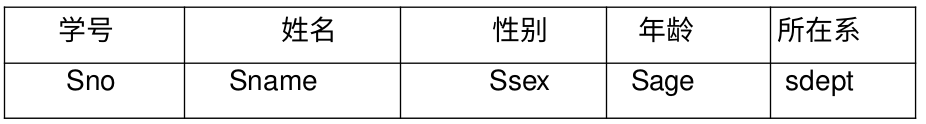
\includegraphics[width=1\textwidth]{ex1-1.png}} % 插入圖片,[] 為圖片大小,{} 是圖片文件
    \subfigure[创建课程关系表C]{
    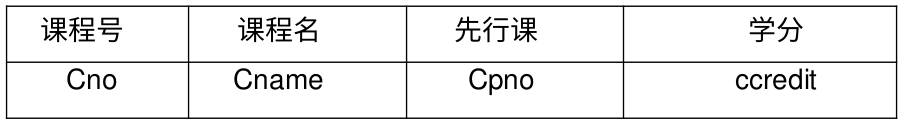
\includegraphics[width=0.8\textwidth]{ex1-2.png}}
    \subfigure[创建学生-课程表SC]{
    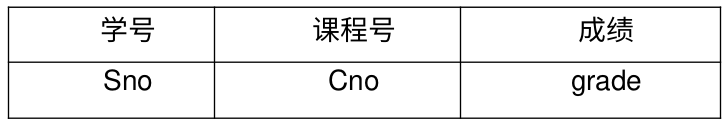
\includegraphics[width=0.75\textwidth]{ex1-3.png}}
\end{figure}

\begin{itemize}
    \item 将以上创建表S、C、SC的SQL命令以 .SQL文件的形式保存在磁盘上。在表中加入至少4个元组,第一个为本人信息。
    \item 在表S上增加“出生日期”与“身高”属性列。
    \item 删除表S的“身高” 属性列。
    \item 备份数据库,再还原。
\end{itemize}

\section{實驗方法與實驗步驟}

\begin{itemize}
    \item 创建数据库或连接已建立的数据库。
    \item 在当前数据库上建立新表。
    \item 定义表的结构。
    \item 修改表的结构。
\end{itemize}

\section{實驗結果}

\subsection{在 ArchLinux 上配置好 MySQL}

\begin{lstlisting}[language=Octave]
    $ sudo pacman -S mariadb # 安裝 mariadb
    $ chattr +C /var/lib/mysql # disabling Copy-on-Write,因為我的文件系統是 Btrfs
    $ systemctl enable mariadb # 啟用
    $ systemctl start mariadb # 執行
    $ sudo mysql -u root -p # 以 root 身份進行
\end{lstlisting}

{可以自己設定一些密碼或是新增使用者}

\subsection{創建 student\_data database}

\begin{figure}[H] % H 為當前位置,!htb 為忽略美學標準,htbp 為浮動圖片
    \centering % 圖片居中
    \subfigure[創建 database]{
    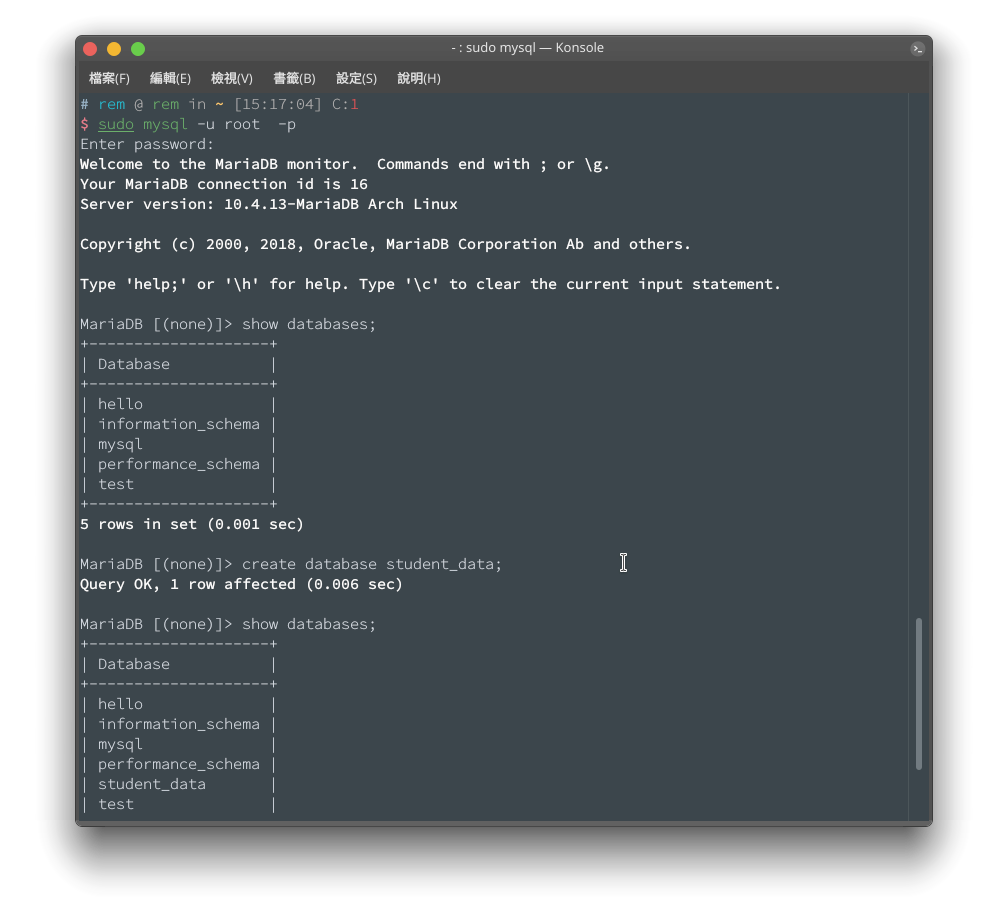
\includegraphics[width=1\textwidth]{ex1-4.png}}
\end{figure}

\subsection{將 Table 創建出來}

{至少每個 Table 填入四筆數據}

\begin{figure}[H] % H 為當前位置,!htb 為忽略美學標準,htbp 為浮動圖片
    \centering % 圖片居中
    \subfigure[創建 Table S]{
    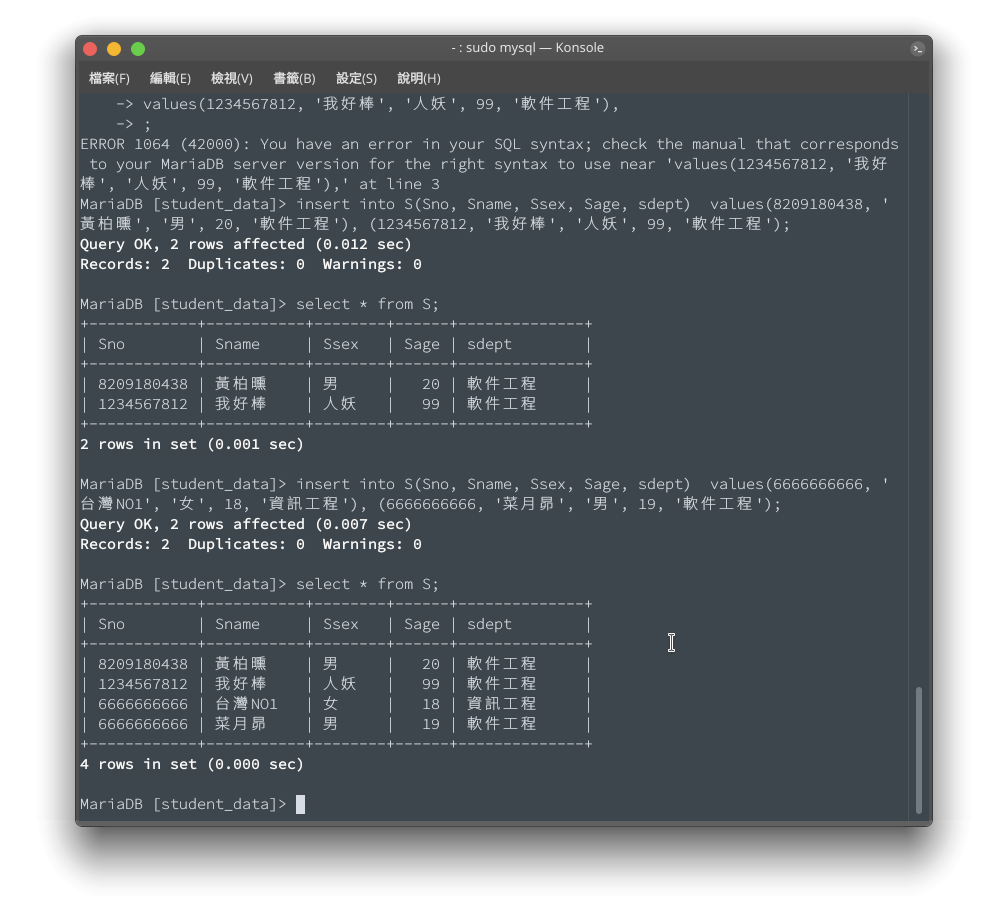
\includegraphics[width=1\textwidth]{ex1-5.png}}
\end{figure}

\begin{figure}[H] % H 為當前位置,!htb 為忽略美學標準,htbp 為浮動圖片
    \centering % 圖片居中
    \subfigure[創建 Table C]{
    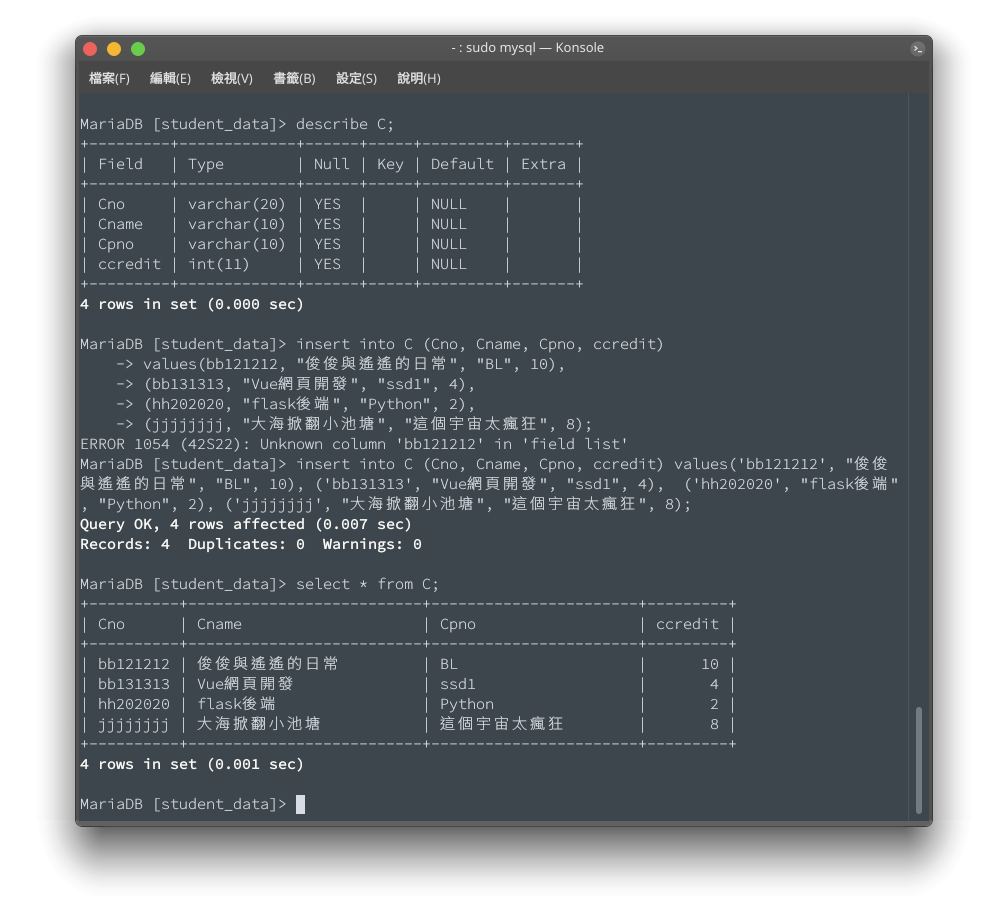
\includegraphics[width=1\textwidth]{ex1-6.png}}
\end{figure}

\begin{figure}[H] % H 為當前位置,!htb 為忽略美學標準,htbp 為浮動圖片
    \centering % 圖片居中
    \subfigure[創建 Table SC]{
    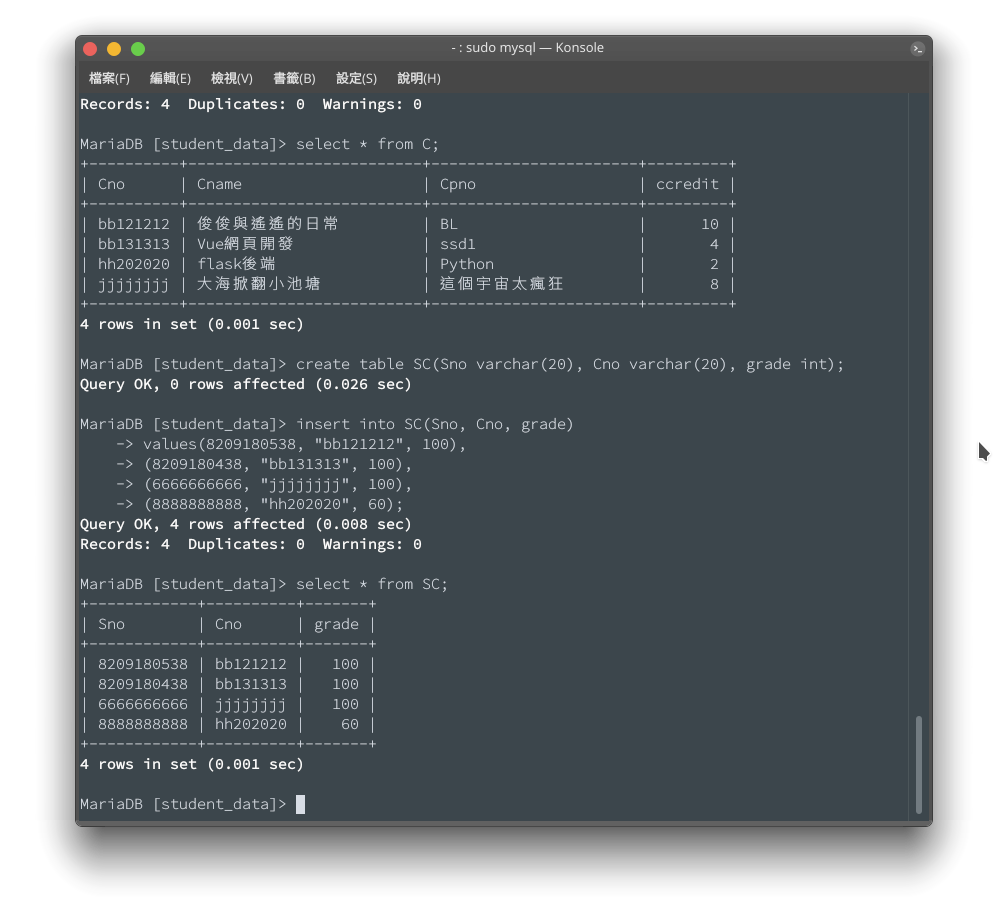
\includegraphics[width=1\textwidth]{ex1-7.png}}
\end{figure}

\subsection{新增屬性列與刪除屬性列}

在 S Table 新增 SBirthday(生日)與 SHeight(身高)。

\begin{figure}[H] % H 為當前位置,!htb 為忽略美學標準,htbp 為浮動圖片
    \centering % 圖片居中
    \subfigure[Table S 添加列]{
    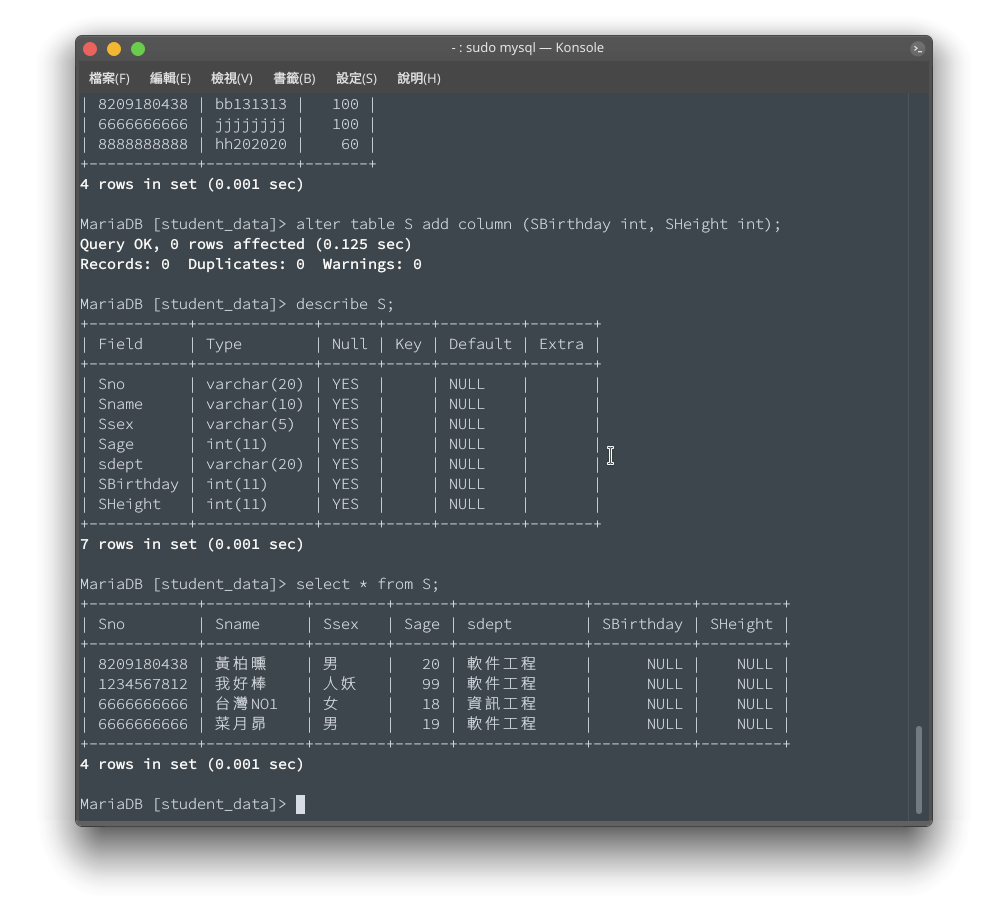
\includegraphics[width=1\textwidth]{ex1-8.png}}
\end{figure}

刪除 S Table 中的 SHeight(身高)。

\begin{figure}[H] % H 為當前位置,!htb 為忽略美學標準,htbp 為浮動圖片
    \centering % 圖片居中
    \subfigure[Table S 刪除列]{
    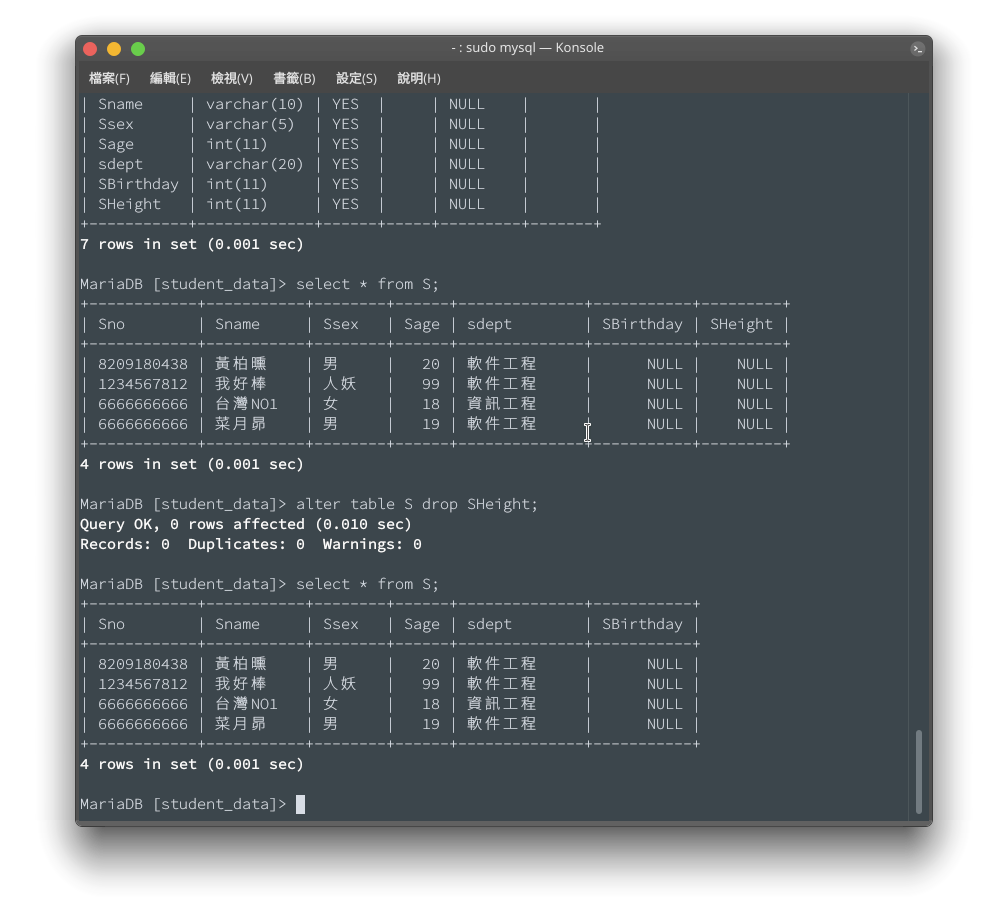
\includegraphics[width=1\textwidth]{ex1-9.png}}
\end{figure}

\subsection{SQL 的備份與還原}

匯出 mySQL 文件

\begin{figure}[H] % H 為當前位置,!htb 為忽略美學標準,htbp 為浮動圖片
    \centering % 圖片居中
    \subfigure[匯出 student\_data.sql 文件]{
    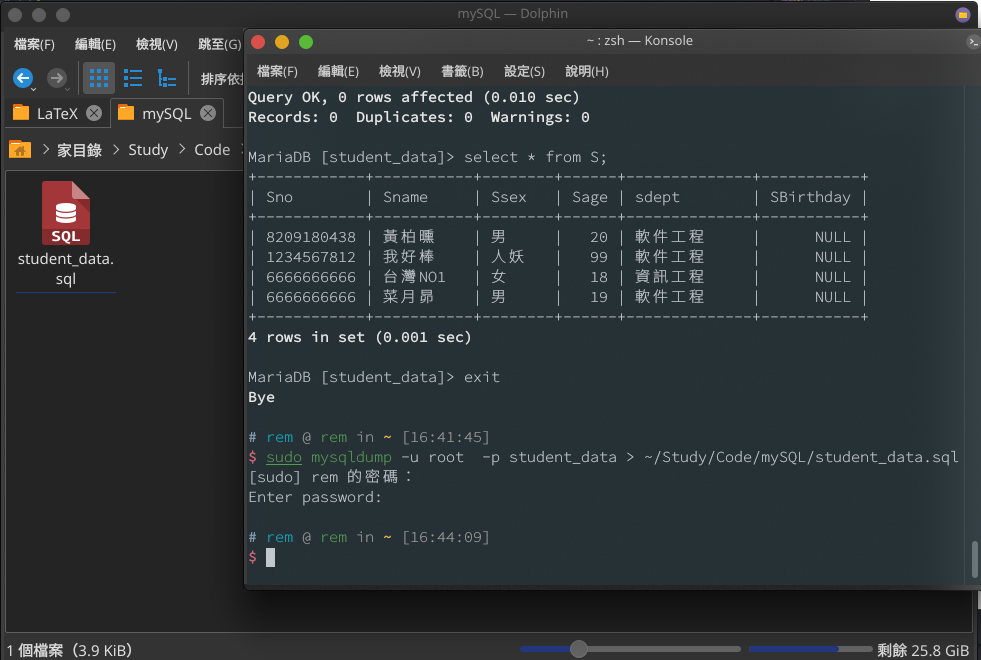
\includegraphics[width=1\textwidth]{ex1-10.png}}
\end{figure}

匯入 mySQL 文件

\begin{figure}[H] % H 為當前位置,!htb 為忽略美學標準,htbp 為浮動圖片
    \centering % 圖片居中
    \subfigure[匯入 student\_data.sql 文件]{
    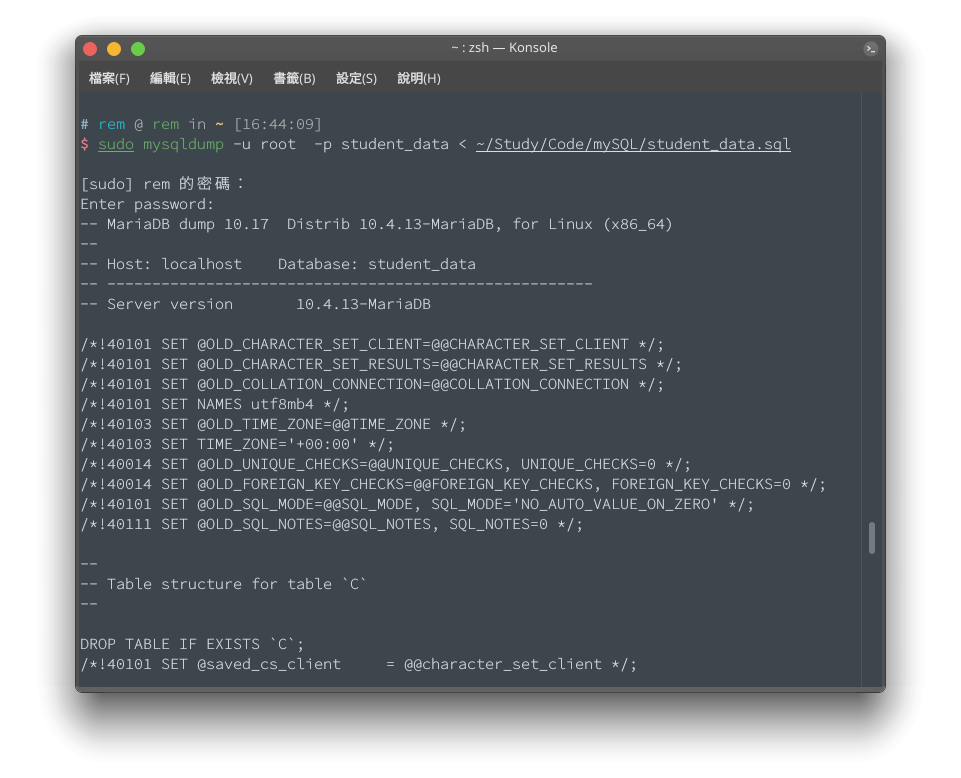
\includegraphics[width=1\textwidth]{ex1-11.png}}
\end{figure}

\begin{figure}[H] % H 為當前位置,!htb 為忽略美學標準,htbp 為浮動圖片
    \centering % 圖片居中
    \subfigure[student\_data 已被還原]{
    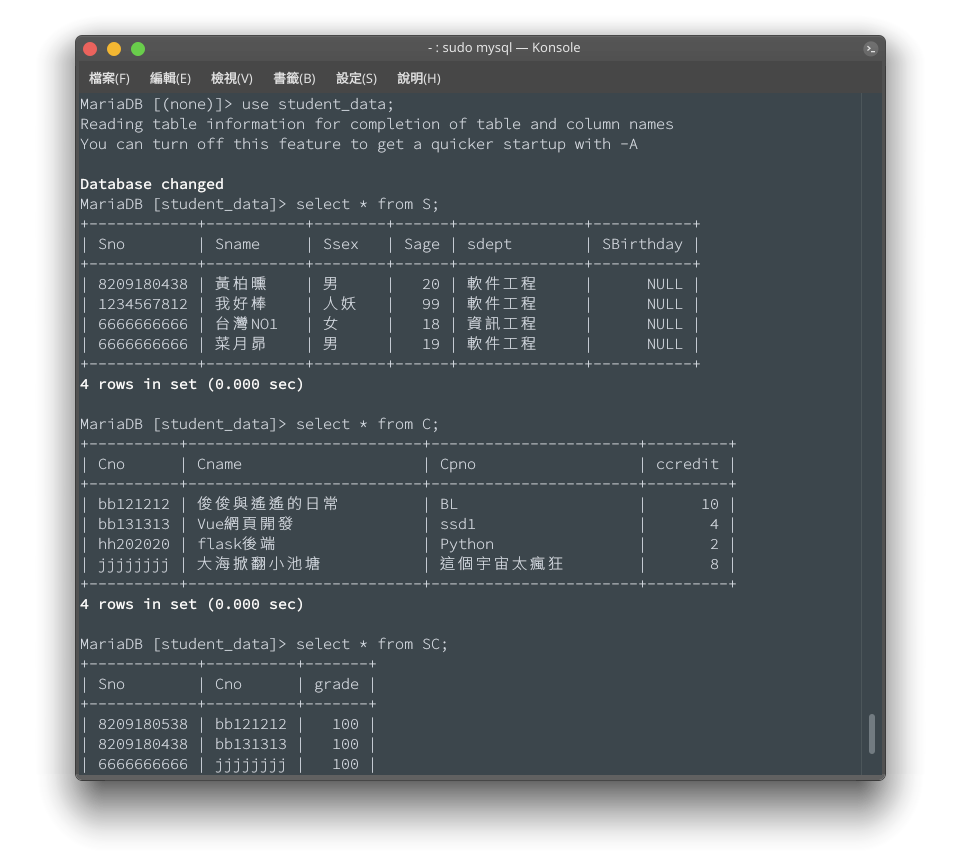
\includegraphics[width=1\textwidth]{ex1-12.png}}
\end{figure}

\section{實驗小結}

本次實驗讓我們學習基本的數據庫操作,讓我們了解數據庫的基本指令,我也在這次實驗學會了怎麼使用數據庫。有時我打指令會忘記在每行指令後面添加分號,造成要重打一次,不過這樣是讓我養成習慣。

\part{實驗二、數據庫查詢與更新}

\section{實驗目的}

\begin{itemize}
    \item 熟悉和掌握对数据表中数据的查询操作和SQL命令的使用,学会灵活熟练的使用SQL 语句的各种形式,加深理解关系运算的各种操作(尤其是关系的选择,投影,连接和除运算);
    \item 熟悉和掌握数据表中数据的插入、修改、删除操作和命令的使用(熟悉使用UPDATE/INSERT/DELETE语句进行表操作);加深理解表的定义对数据更新的作用。
\end{itemize}

\section{實驗內容}

\subsection{在表S,C,SC上完成以下查询}

\begin{itemize}
    \item 查询学生的基本信息;
    \item 查询“CS”系学生的基本信息;
    \item 查询“CS”系学生年龄不在19到21之间的学生的学号、姓名;
    \item 找出“CS”系年龄最大的学生,显示其学号、姓名;
    \item 找出各系年龄最大的学生,显示其学号、姓名;
    \item 统计“CS”系学生的人数;
    \item 统计各系学生的人数,结果按升序排列;
    \item 按系统计各系学生的平均年龄,结果按降序排列;
    \item 查询无先修课的课程的课程名和学时数;
    \item 统计每位学生选修课程的门数、学分及其平均成绩;
    \item 统计选修每门课程的学生人数及各门课程的平均成绩;
    \item 找出平均成绩在85分以上的学生,结果按系分组,并按平均成绩的升序排列;
    \item 查询选修了“1”或“2”号课程的学生学号和姓名;
    \item 查询选修了课程名为“数据库系统”且成绩在60分以下的学生的学号、姓名和成绩;
    \item 查询每位学生选修了课程的学生信息(显示:学号,姓名,课程号,课程名,成绩);
    \item 查询没有选修课程的学生的基本信息;
    \item 查询选修了3门以上课程的学生学号;
    \item 查询选修课程成绩至少有一门在80分以上的学生学号;
    \item 查询选修课程成绩均在80分以上的学生学号;
\end{itemize}

\subsection{在表S、C、SC中完成下列更新}

\begin{itemize}
    \item 将数据分别插入表S、C、SC;
    \item 将表S、C、SC中的数据保存在磁盘上。
    \item 在表S、C、SC上练习数据的插入、修改、删除操作。(比较在表上定义/未定义主码(Primary Key)或外码(Foreign Key)时的情况)
    \item 将表S、C、SC中的数据全部删除,再利用磁盘上备份的数据来恢复数据。
    \item 如果要在表SC中插入某个学生的选课信息(如:学号为“2007001005”,课程号为“c123”,成绩待定),应如何进行?
    \item 求各系学生的平均成绩,并把结果存入数据库;
    \item 将“CS”系全体学生的成绩置零;
    \item 删除“CS”系全体学生的选课记录;
    \item 删除学号为“S1”的相关信息;
    \item 将学号为“S1”的学生的学号修改为“S001”;
    \item 把平均成绩大于80分的男同学的学号和平均成绩存入另一个表S——GRADE(SNO,AVG\_GRADE);
    \item 把选修了课程名为“数据结构”的学生的成绩提高10%;
    \item 把选修了“C2”号课程,且成绩低于该门课程的平均成绩的学生成绩删除掉。
\end{itemize}

\section{實驗方法與實驗步驟}

\subsection{查询}

\begin{itemize}
    \item 在表S、C、SC上进行简单查询、连接查询、嵌套查询;
    \item 使用聚合函数的查询、对数据分组查询、对数据的排序查询。
\end{itemize}

\subsection{插入}

\begin{itemize}
    \item 用SQL命令将数据插入当前数据库的表S、C、SC中;
    \item 用SQL命令形式修改表S、C、SC中的数据;
    \item 用SQL命令形式  删除表S、C、SC中的数据。
\end{itemize}

\section{實驗結果}

\subsection{查詢}

1. 查詢學生的基本訊息\\

\begin{lstlisting}[language=SQL]
    select * from S;
\end{lstlisting}

\begin{figure}[H] % H 為當前位置,!htb 為忽略美學標準,htbp 為浮動圖片
    \centering % 圖片居中
    \subfigure[查询学生的基本信息]{
    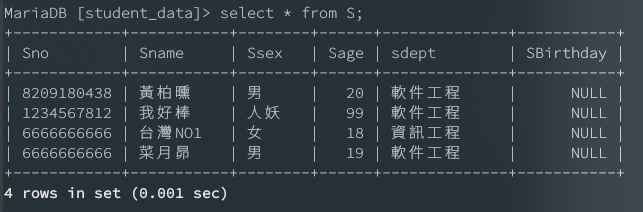
\includegraphics[width=1\textwidth]{ex2-1.png}}
\end{figure}
% ----------------------------------------------------------
2. 查询“CS”系学生的基本信息\\

\begin{lstlisting}[language=SQL]
    select * from S where sdept='資訊工程';
\end{lstlisting}

\begin{figure}[H] % H 為當前位置,!htb 為忽略美學標準,htbp 為浮動圖片
    \centering % 圖片居中
    \subfigure[查询“CS”系学生的基本信息]{
    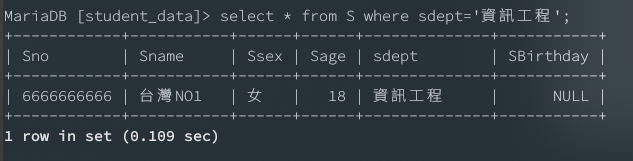
\includegraphics[width=1\textwidth]{ex2-2.png}}
\end{figure}
% ----------------------------------------------------------
3. 查询“CS”系学生年龄不在19到21之间的学生的学号、姓名。\\

\begin{lstlisting}[language=SQL]
    select Sno, Sname from S where sdept='資訊工程' and Sage not between 19 and 21;
\end{lstlisting}

\begin{figure}[H] % H 為當前位置,!htb 為忽略美學標準,htbp 為浮動圖片
    \centering % 圖片居中
    \subfigure[查询“CS”系学生年龄不在19到21之间的学生的学号、姓名]{
    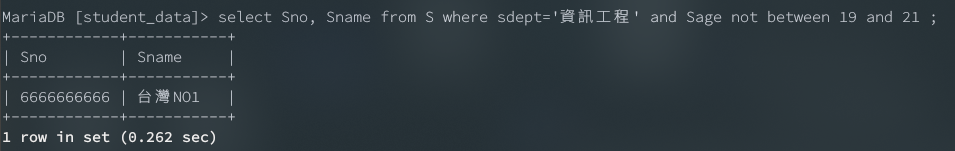
\includegraphics[width=1\textwidth]{ex2-3.png}}
\end{figure}
% ----------------------------------------------------------
4. 找出“CS”系年龄最大的学生,显示其学号、姓名。

這題有難度

這裡我為了實驗的操作性,將 "CS" 變成"軟件工程"。\\

\begin{lstlisting}[language=SQL]
    select Sno, Sname from (select max(Sage) as Sage, Sno, Sname from S where sdept='軟件工程');
\end{lstlisting}

\begin{figure}[H] % H 為當前位置,!htb 為忽略美學標準,htbp 為浮動圖片
    \centering % 圖片居中
    \subfigure[找出“CS”系年龄最大的学生,显示其学号、姓名]{
    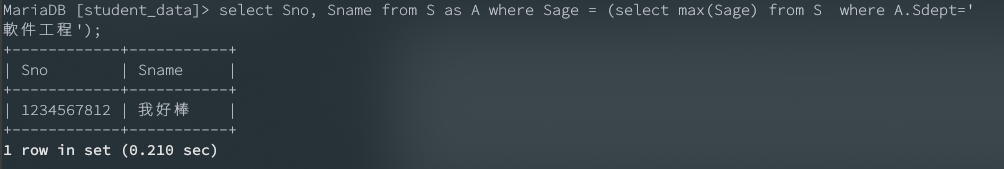
\includegraphics[width=1\textwidth]{ex2-4.png}}
\end{figure}
% ----------------------------------------------------------
5. 找出各系年龄最大的学生,显示其学号、姓名。\\

\begin{lstlisting}[language=SQL]
    select Sno, Sname from S as A where Sage = (select max(Sage) from S as B where A.Sdept = B.Sdept);
\end{lstlisting}

\begin{figure}[H] % H 為當前位置,!htb 為忽略美學標準,htbp 為浮動圖片
    \centering % 圖片居中
    \subfigure[找出各系年龄最大的学生,显示其学号、姓名]{
    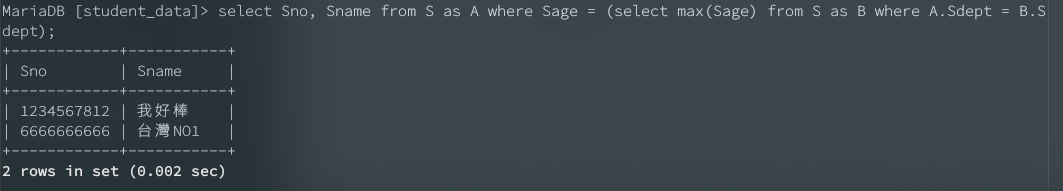
\includegraphics[width=1\textwidth]{ex2-5.png}}
\end{figure}
% ----------------------------------------------------------
6. 统计“CS”系学生的人数。\\

\begin{lstlisting}[language=SQL]
    select count(Sdept) from S where Sdept="軟件工程";
\end{lstlisting}

\begin{figure}[H] % H 為當前位置,!htb 為忽略美學標準,htbp 為浮動圖片
    \centering % 圖片居中
    \subfigure[统计“CS”系学生的人数]{
    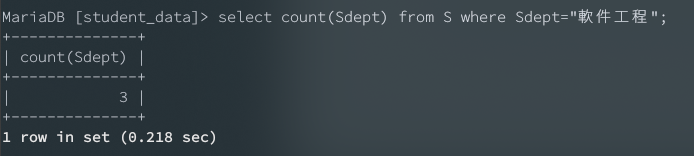
\includegraphics[width=1\textwidth]{ex2-6.png}}
\end{figure}

% ----------------------------------------------------------
7. 统计各系学生的人数,结果按升序排列。\\

\begin{lstlisting}[language=SQL]
    select Sdept, count(Sdept) as Sum from S group by Sdept order by Sum;
\end{lstlisting}

\begin{figure}[H] % H 為當前位置,!htb 為忽略美學標準,htbp 為浮動圖片
    \centering % 圖片居中
    \subfigure[统计各系学生的人数,结果按升序排列]{
    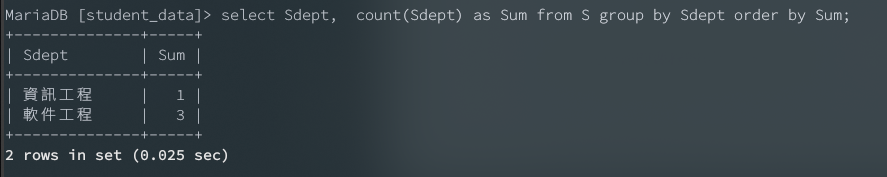
\includegraphics[width=1\textwidth]{ex2-7.png}}
\end{figure}

% ----------------------------------------------------------
8. 按系统计各系学生的平均年龄,结果按降序排列。\\

\begin{lstlisting}[language=SQL]
    select Sdept, avg(Sage) as Age from S group by Sdept order by Age DESC;
\end{lstlisting}

\begin{figure}[H] % H 為當前位置,!htb 為忽略美學標準,htbp 為浮動圖片
    \centering % 圖片居中
    \subfigure[按系统计各系学生的平均年龄,结果按降序排列]{
    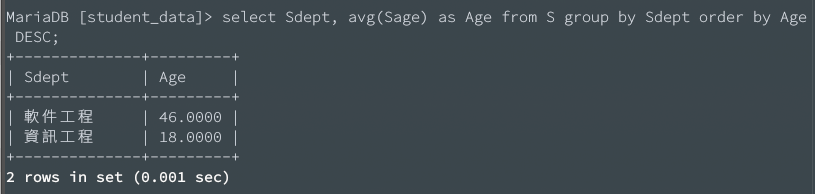
\includegraphics[width=1\textwidth]{ex2-8.png}}
\end{figure}

% ----------------------------------------------------------
9. 查询无先修课的课程的课程名和学时数。

因為實驗一的 C Table 我沒添加無先修課的數據,所以在這裡添加了一筆沒有先修課程的數據。\\

\begin{lstlisting}[language=SQL]
    insert into C(Cno, Cname, Cpno, ccredit) values('rrrrrrrr', '我沒有先修課', null, 100);
    select Cname, ccredit from C where Cpno is null;
\end{lstlisting}

\begin{figure}[H] % H 為當前位置,!htb 為忽略美學標準,htbp 為浮動圖片
    \centering % 圖片居中
    \subfigure[插入一筆數據]{
    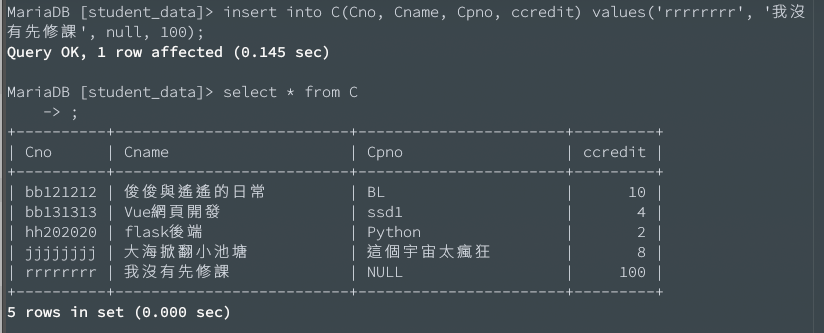
\includegraphics[width=1\textwidth]{ex2-9.png}}
\end{figure}


\begin{figure}[H] % H 為當前位置,!htb 為忽略美學標準,htbp 為浮動圖片
    \centering % 圖片居中
    \subfigure[查询无先修课的课程的课程名和学时数]{
    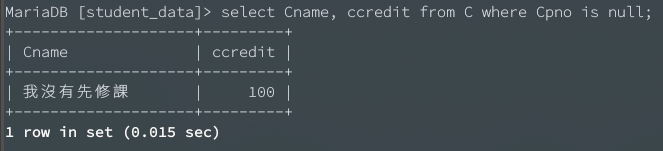
\includegraphics[width=1\textwidth]{ex2-10.png}}
\end{figure}

% ----------------------------------------------------------
10. 统计每位学生选修课程的门数、学分及其平均成绩。\\

\begin{lstlisting}[language=SQL]
    select Sno, count(Cno), avg(grade) from SC as A where Sno = (select Sno from SC as B where A.Sno = B.Sno)  group by Sno;
\end{lstlisting}

\begin{figure}[H] % H 為當前位置,!htb 為忽略美學標準,htbp 為浮動圖片
    \centering % 圖片居中
    \subfigure[统计每位学生选修课程的门数、学分及其平均成绩]{
    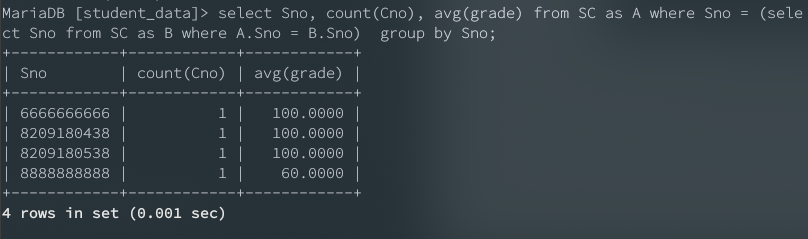
\includegraphics[width=1\textwidth]{ex2-11.png}}
\end{figure}

% ----------------------------------------------------------
11. 统计选修每门课程的学生人数及各门课程的平均成绩。\\

\begin{lstlisting}[language=SQL]
    select Cno, count(Sno), avg(grade) from SC as A where Cno = (select Cno from SC as B where A.Cno = B.Cno)  group by Cno;
\end{lstlisting}

\begin{figure}[H] % H 為當前位置,!htb 為忽略美學標準,htbp 為浮動圖片
    \centering % 圖片居中
    \subfigure[统计每位学生选修课程的门数、学分及其平均成绩]{
    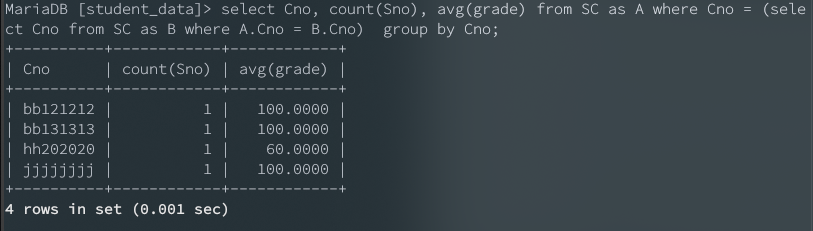
\includegraphics[width=1\textwidth]{ex2-12.png}}
\end{figure}

% ----------------------------------------------------------
12. 找出平均成绩在85分以上的学生,结果按系分组,并按平均成绩的升序排列。\\

\begin{lstlisting}[language=SQL]
    select S.Sno, S.sdept, AVG(SC.grade) from SC, S where SC.Sno = S.Sno group by S.Sno, S.sdept having avg(SC.grade) > 85 order by AVG(SC.grade) ASC;
\end{lstlisting}

\begin{figure}[H] % H 為當前位置,!htb 為忽略美學標準,htbp 為浮動圖片
    \centering % 圖片居中
    \subfigure[找出平均成绩在85分以上的学生,结果按系分组,并按平均成绩的升序排列]{
    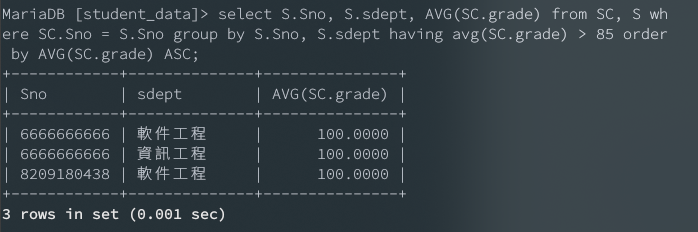
\includegraphics[width=1\textwidth]{ex2-13.png}}
\end{figure}

% ----------------------------------------------------------
13. 查询选修了“1”或“2”号课程的学生学号和姓名。

我在這裡因為沒有 "1" 和 "2" 的課程,所以改成數據庫有的。\\


\begin{lstlisting}[language=SQL]
    select SC.Sno, S.Sname from SC, S where SC.Cno = "bb121212" and SC.Sno union select SC.Sno, S.Sname from SC, S where SC.Cno = "bb131313" and SC.Sno = S.Sno;
\end{lstlisting}

\begin{figure}[H] % H 為當前位置,!htb 為忽略美學標準,htbp 為浮動圖片
    \centering % 圖片居中
    \subfigure[查询选修了“1”或“2”号课程的学生学号和姓名]{
    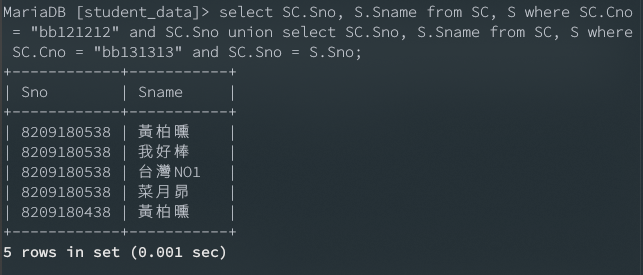
\includegraphics[width=1\textwidth]{ex2-14.png}}
\end{figure}

% ----------------------------------------------------------
14. 查询选修了课程名为“数据库系统”且成绩在60分以下的学生的学号、姓名和成绩。\\

\begin{lstlisting}[language=SQL]
    select SC.Sno, Sname, grade from SC, S, C where SC.sno = S.Sno and SC.Cno = C.Cno and Cname = 'SSD7' and grade < 60;
\end{lstlisting}

\begin{figure}[H] % H 為當前位置,!htb 為忽略美學標準,htbp 為浮動圖片
    \centering % 圖片居中
    \subfigure[查询选修了课程名为“数据库系统”且成绩在60分以下的学生的学号、姓名和成绩]{
    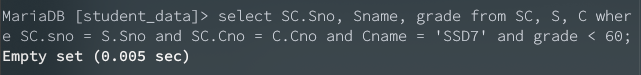
\includegraphics[width=1\textwidth]{ex2-15.png}}
\end{figure}

% ----------------------------------------------------------
15. 查询每位学生选修了课程的学生信息(显示:学号,姓名,课程号,课程名,成绩)。\\

\begin{lstlisting}[language=SQL]
    select SC.Sno, Sname, C.Cno, Cname, grade from SC, S, C where SC.Sno = S.Sno and SC.cno = C.cno;
\end{lstlisting}

\begin{figure}[H] % H 為當前位置,!htb 為忽略美學標準,htbp 為浮動圖片
    \centering % 圖片居中
    \subfigure[查询每位学生选修了课程的学生信息(显示:学号,姓名,课程号,课程名,成绩)]{
    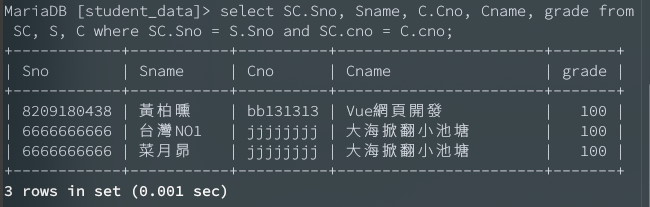
\includegraphics[width=1\textwidth]{ex2-16.png}}
\end{figure}

% ----------------------------------------------------------
16. 查询没有选修课程的学生的基本信息。\\

\begin{lstlisting}[language=SQL]
    select * from S where S.Sno not in(select SC.Sno from S, SC where SC.Sno = S.Sno);
\end{lstlisting}

\begin{figure}[H] % H 為當前位置,!htb 為忽略美學標準,htbp 為浮動圖片
    \centering % 圖片居中
    \subfigure[查询没有选修课程的学生的基本信息]{
    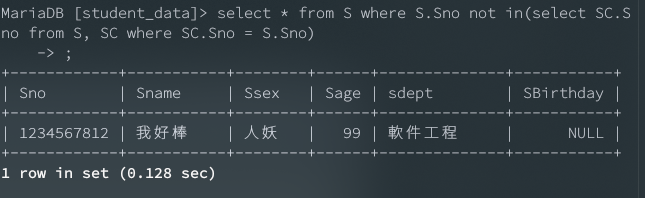
\includegraphics[width=1\textwidth]{ex2-17.png}}
\end{figure}

% ----------------------------------------------------------
17. 查询选修了3门以上课程的学生学号。\\

\begin{lstlisting}[language=SQL]
    select Sno from SC group by Sno having count(Cno) > 3;
\end{lstlisting}

\begin{figure}[H] % H 為當前位置,!htb 為忽略美學標準,htbp 為浮動圖片
    \centering % 圖片居中
    \subfigure[查询选修了3门以上课程的学生学号]{
    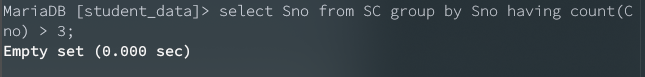
\includegraphics[width=1\textwidth]{ex2-18.png}}
\end{figure}

% ----------------------------------------------------------
18. 查询选修课程成绩至少有一门在80分以上的学生学号。\\

\begin{lstlisting}[language=SQL]
    select distinct Sno from SC where grade > 80;
\end{lstlisting}

\begin{figure}[H] % H 為當前位置,!htb 為忽略美學標準,htbp 為浮動圖片
    \centering % 圖片居中
    \subfigure[查询选修课程成绩至少有一门在80分以上的学生学号]{
    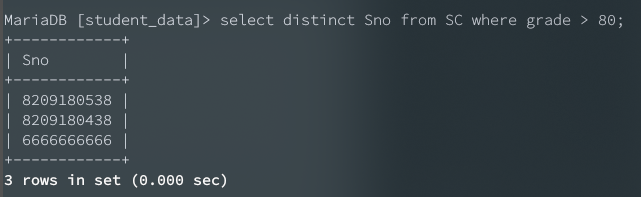
\includegraphics[width=1\textwidth]{ex2-19.png}}
\end{figure}

% ----------------------------------------------------------
19. 查询选修课程成绩均在80分以上的学生学号。\\

\begin{lstlisting}[language=SQL]
    select SC.Sno from SC where SC.grade > 80;
\end{lstlisting}

\begin{figure}[H] % H 為當前位置,!htb 為忽略美學標準,htbp 為浮動圖片
    \centering % 圖片居中
    \subfigure[查询选修课程成绩均在80分以上的学生学号]{
    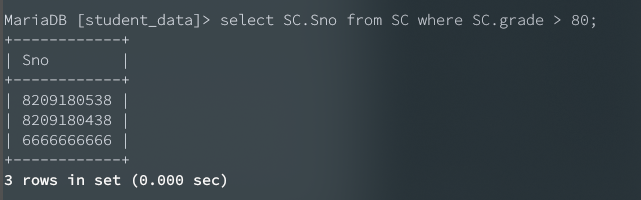
\includegraphics[width=1\textwidth]{ex2-20.png}}
\end{figure}

\subsection{更新}

1. 将数据分别插入表S、C、SC。\\

\begin{figure}[H] % H 為當前位置,!htb 為忽略美學標準,htbp 為浮動圖片
    \centering % 圖片居中
    \subfigure[創建 Table S]{
    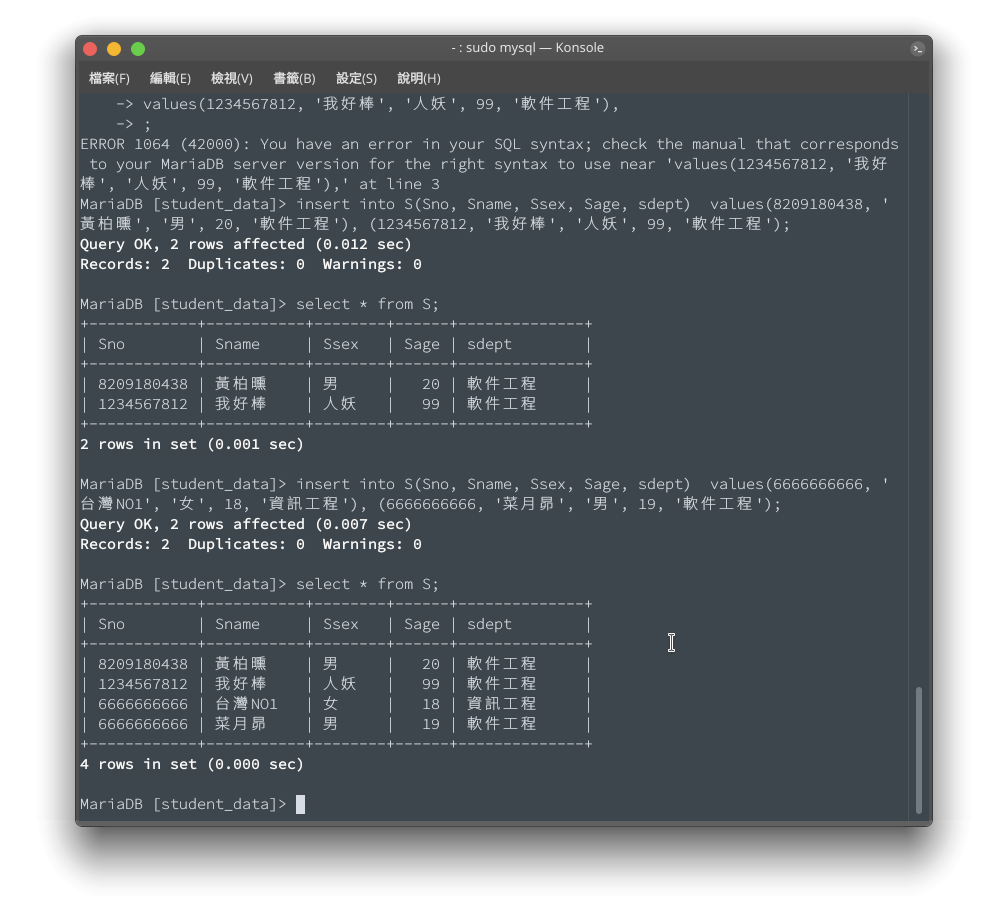
\includegraphics[width=1\textwidth]{ex1-5.png}}
\end{figure}

\begin{figure}[H] % H 為當前位置,!htb 為忽略美學標準,htbp 為浮動圖片
    \centering % 圖片居中
    \subfigure[創建 Table C]{
    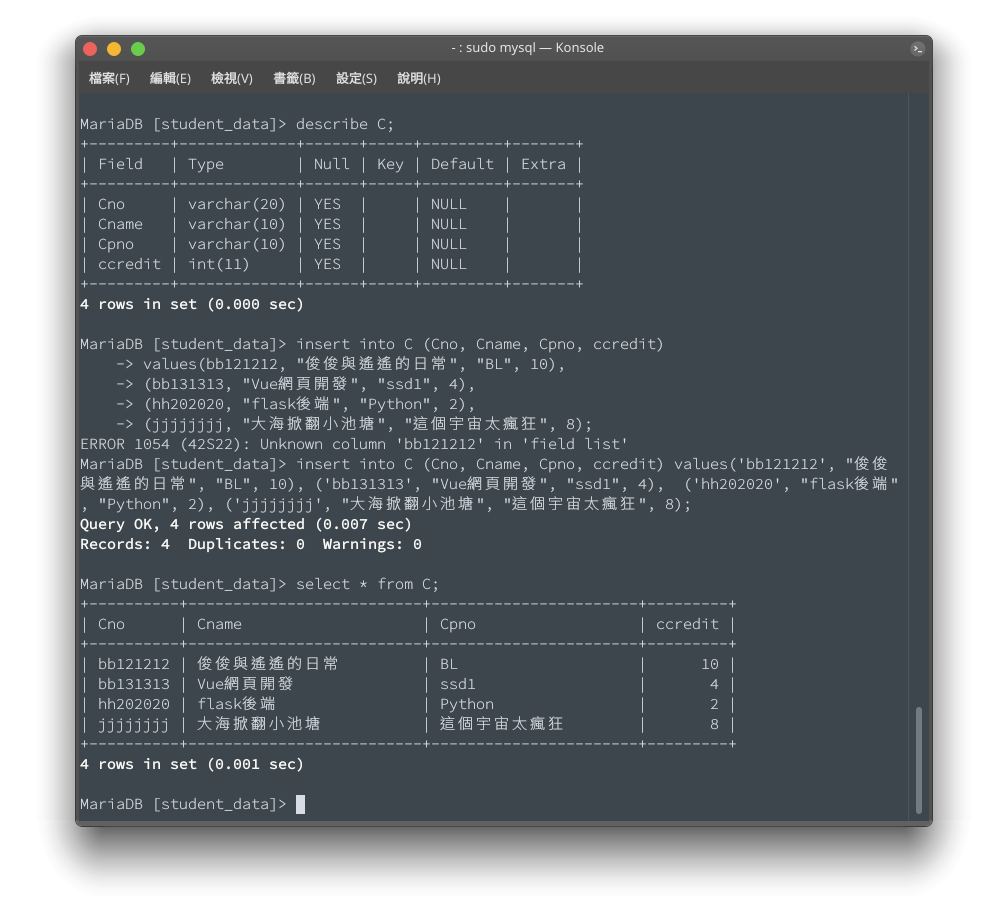
\includegraphics[width=1\textwidth]{ex1-6.png}}
\end{figure}

\begin{figure}[H] % H 為當前位置,!htb 為忽略美學標準,htbp 為浮動圖片
    \centering % 圖片居中
    \subfigure[創建 Table SC]{
    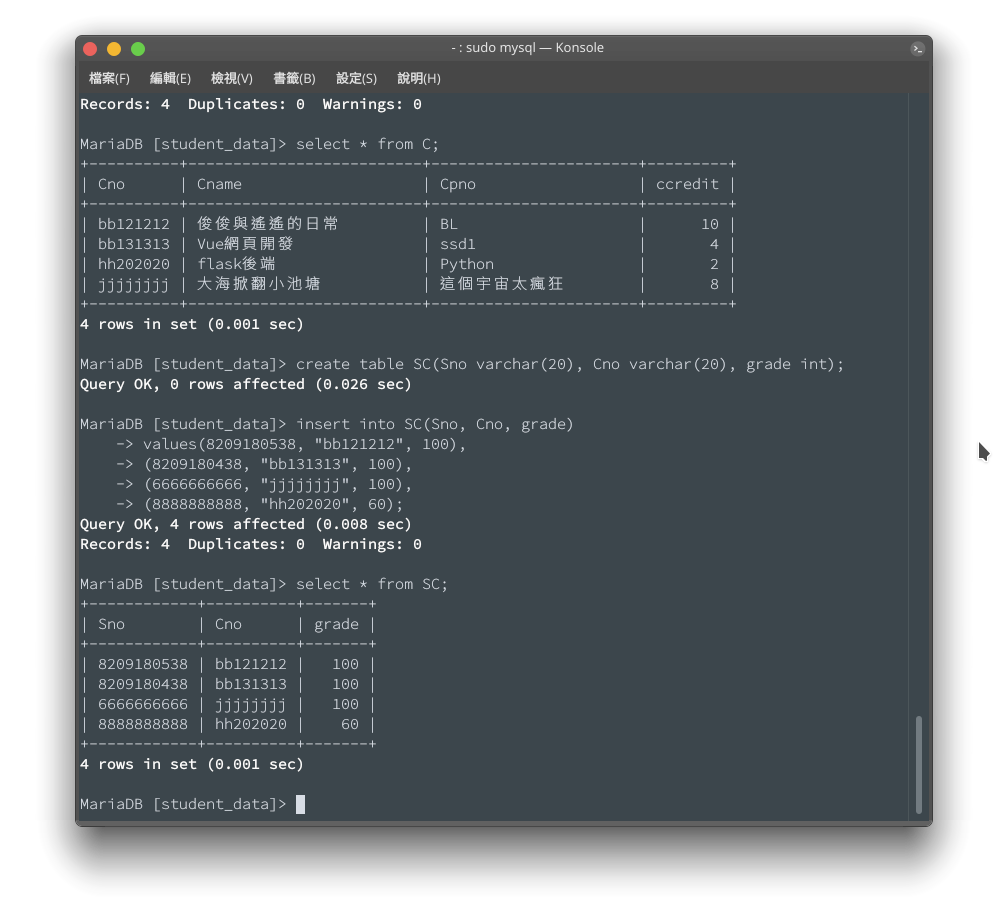
\includegraphics[width=1\textwidth]{ex1-7.png}}
\end{figure}

% -------------------------------------------------------------------
2. 将表S、C、SC中的数据保存在磁盘上。

\begin{figure}[H] % H 為當前位置,!htb 為忽略美學標準,htbp 為浮動圖片
    \centering % 圖片居中
    \subfigure[匯出 student\_data.sql 文件]{
    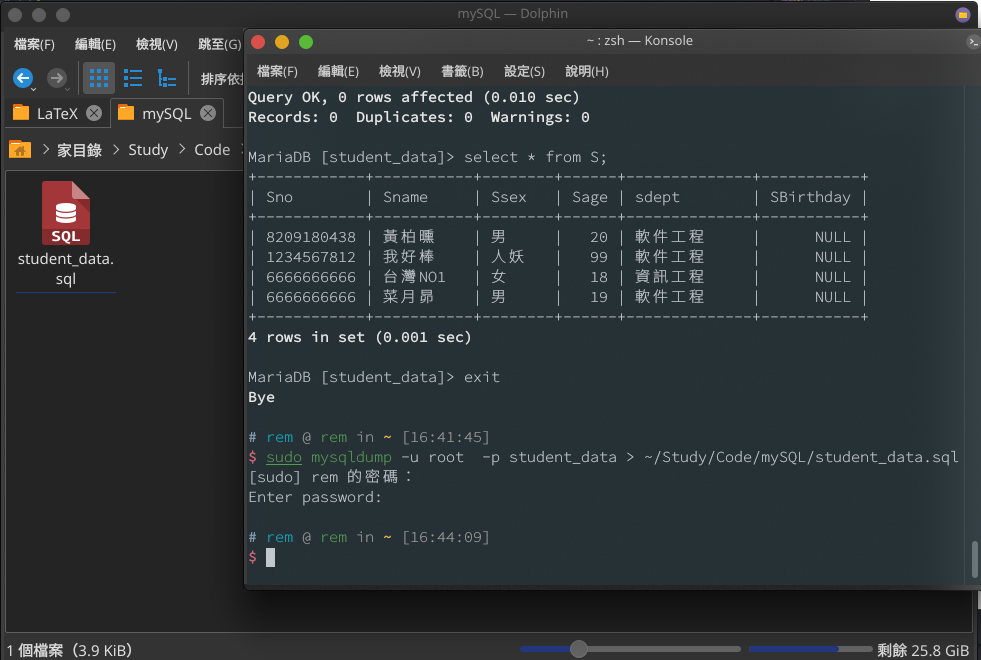
\includegraphics[width=1\textwidth]{ex1-10.png}}
\end{figure}

% -------------------------------------------------------------------
3. 在表S、C、SC上练习数据的插入、修改、删除操作。(比较在表上定义/未定义主码(Primary Key)或外码(Foreign Key)时的情况)。\\

\begin{lstlisting}[language=SQL]
    update S set Sname="阿俊" where Sname="菜月昴";
\end{lstlisting}

\begin{figure}[H] % H 為當前位置,!htb 為忽略美學標準,htbp 為浮動圖片
    \centering % 圖片居中
    \subfigure[更新一筆數據]{
    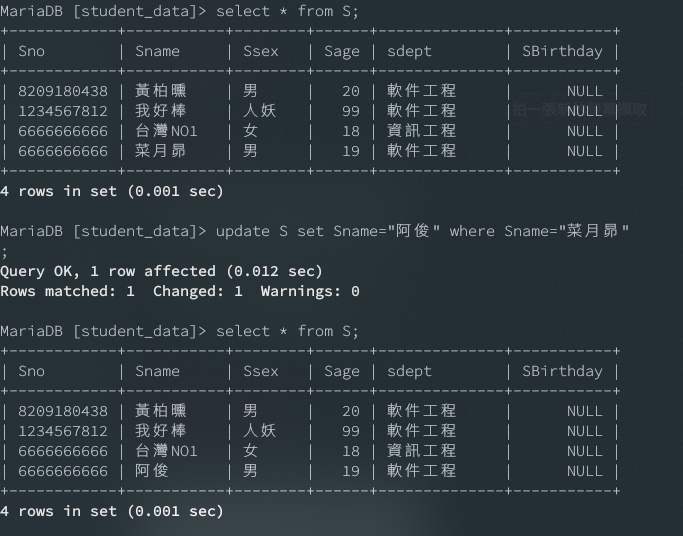
\includegraphics[width=1\textwidth]{ex2-21.png}}
\end{figure}

\begin{lstlisting}[language=SQL]
    alter table S add primary key (Sno);
\end{lstlisting}

\begin{figure}[H] % H 為當前位置,!htb 為忽略美學標準,htbp 為浮動圖片
    \centering % 圖片居中
    \subfigure[設主鍵]{
    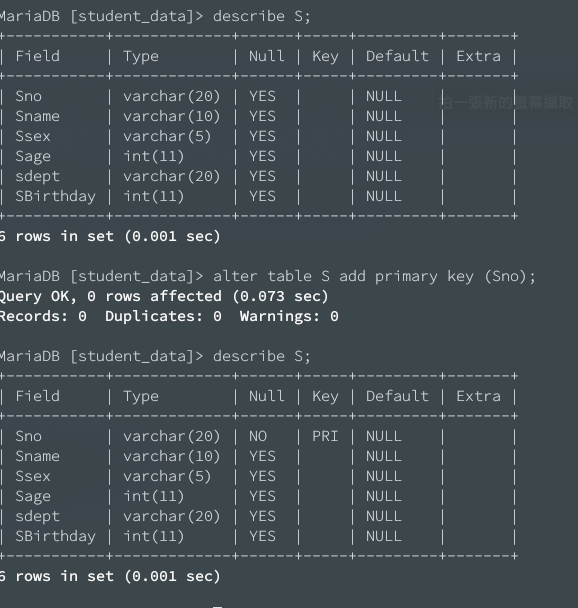
\includegraphics[width=1\textwidth]{ex2-22.png}}
\end{figure}

{設主鍵後,該 Value 不能為 NULL。}\\

% -------------------------------------------------------------------
4. 将表S、C、SC中的数据全部删除,再利用磁盘上备份的数据来恢复数据。\\

\begin{lstlisting}[language=SQL]
    drop table C;
\end{lstlisting}

\begin{figure}[H] % H 為當前位置,!htb 為忽略美學標準,htbp 為浮動圖片
    \centering % 圖片居中
    \subfigure[刪除某個資料表]{
    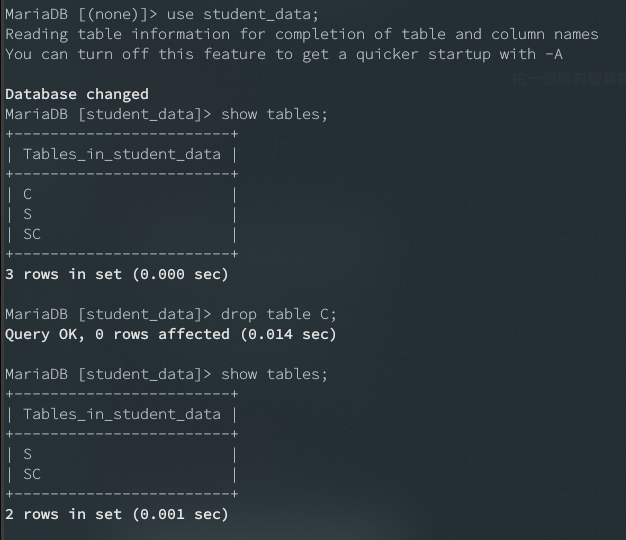
\includegraphics[width=1\textwidth]{ex2-23.png}}
\end{figure}

\begin{lstlisting}[language=Octave]
    mysqldump -u root  -p student_data < ~/Study/Code/mySQL/student_data.sql
\end{lstlisting}

\begin{figure}[H] % H 為當前位置,!htb 為忽略美學標準,htbp 為浮動圖片
    \centering % 圖片居中
    \subfigure[還原整個 Database]{
    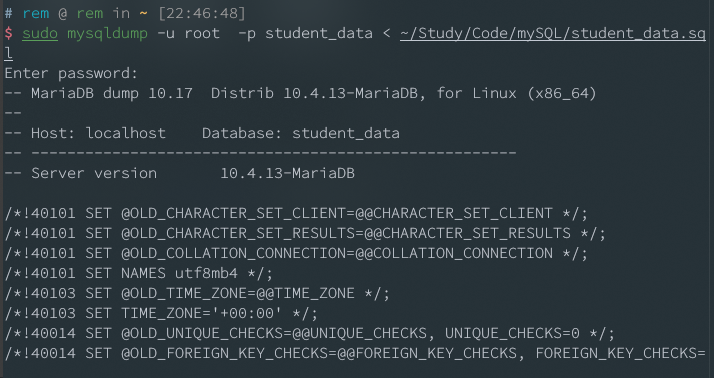
\includegraphics[width=1\textwidth]{ex2-24.png}}
\end{figure}

% -------------------------------------------------------------------
5. 如果要在表SC中插入某个学生的选课信息(如:学号为“2007001005”,课程号为“c123”,成绩待定),应如何进行?\\

\begin{lstlisting}[language=SQL]
    insert into SC (Sno, Cno, grade) values("2007001005", "c123", NULL);
\end{lstlisting}

\begin{figure}[H] % H 為當前位置,!htb 為忽略美學標準,htbp 為浮動圖片
    \centering % 圖片居中
    \subfigure[插入資料]{
    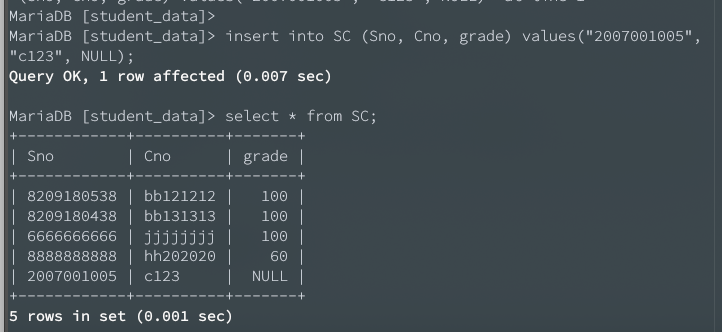
\includegraphics[width=1\textwidth]{ex2-25.png}}
\end{figure}

% -------------------------------------------------------------------
6. 求各系学生的平均成绩,并把结果存入数据库。
因為我不會一次就搞定的指令,所以只好一個一個輸。\\

\begin{lstlisting}[language=SQL]
    select avg(grade) from SC;
    insert SC(Sno, Cno, grade) values("總平均", "-", 90);
\end{lstlisting}

\begin{figure}[H] % H 為當前位置,!htb 為忽略美學標準,htbp 為浮動圖片
    \centering % 圖片居中
    \subfigure[將平均成績插入資料]{
    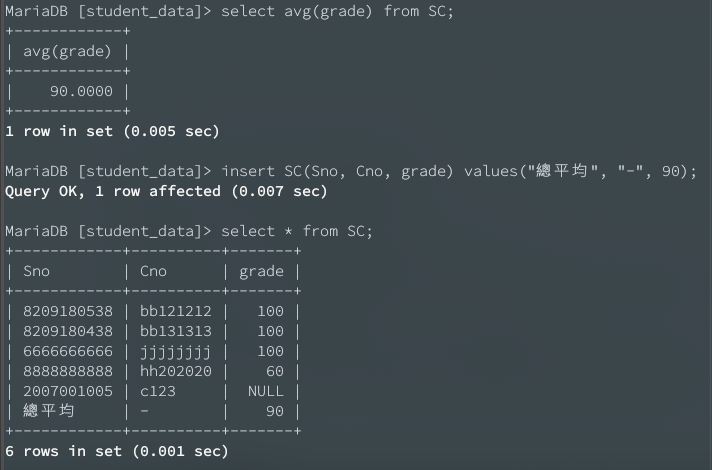
\includegraphics[width=1\textwidth]{ex2-26.png}}
\end{figure}

% -------------------------------------------------------------------
7. 将“CS”系全体学生的成绩置零。\\

\begin{lstlisting}[language=SQL]
    update SC set grade=0 where Sno in (select SC.Sno from SC, S where SC.Sno=S.Sno and S.sdept="軟件工程");
\end{lstlisting}

\begin{figure}[H] % H 為當前位置,!htb 為忽略美學標準,htbp 為浮動圖片
    \centering % 圖片居中
    \subfigure[将“CS”系全体学生的成绩置零]{
    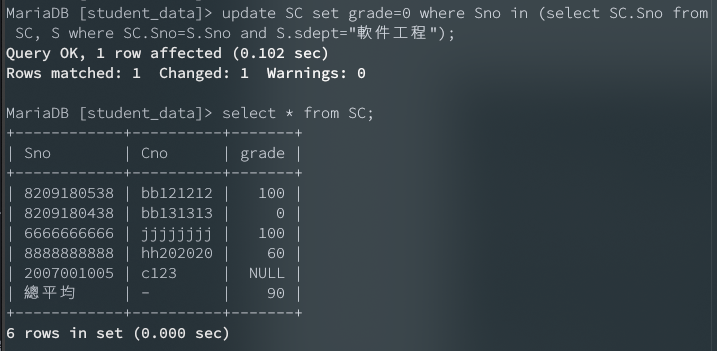
\includegraphics[width=1\textwidth]{ex2-27.png}}
\end{figure}

% -------------------------------------------------------------------
8. 删除“CS”系全体学生的选课记录。\\

\begin{lstlisting}[language=SQL]
    delete from SC where "軟件工程"=(select sdept from S where S.Sno = SC.Sno);
\end{lstlisting}

\begin{figure}[H] % H 為當前位置,!htb 為忽略美學標準,htbp 為浮動圖片
    \centering % 圖片居中
    \subfigure[删除“CS”系全体学生的选课记录]{
    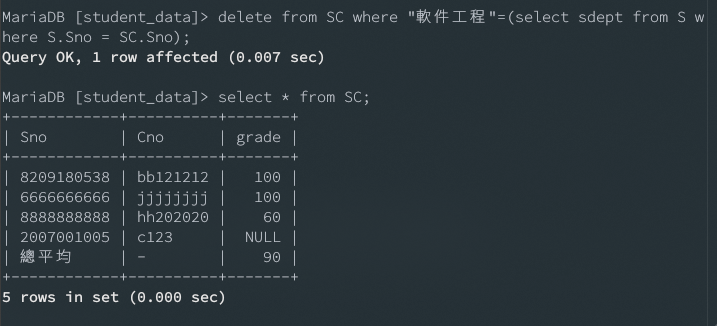
\includegraphics[width=1\textwidth]{ex2-28.png}}
\end{figure}

% -------------------------------------------------------------------
9. 删除学号为“S1”的相关信息。\\

\begin{lstlisting}[language=SQL]
    delete from S where S.Sno="S1";
\end{lstlisting}

\begin{figure}[H] % H 為當前位置,!htb 為忽略美學標準,htbp 為浮動圖片
    \centering % 圖片居中
    \subfigure[删除学号为“S1”的相关信息]{
    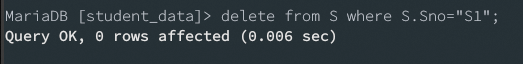
\includegraphics[width=1\textwidth]{ex2-29.png}}
\end{figure}
% -------------------------------------------------------------------
10. 将学号为“S1”的学生的学号修改为“S001”。\\

\begin{lstlisting}[language=SQL]
    update S set Sno="S001" where Sno="S1";
\end{lstlisting}

\begin{figure}[H] % H 為當前位置,!htb 為忽略美學標準,htbp 為浮動圖片
    \centering % 圖片居中
    \subfigure[将学号为“S1”的学生的学号修改为“S001”]{
    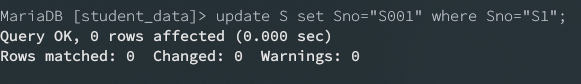
\includegraphics[width=1\textwidth]{ex2-30.png}}
\end{figure}

% -------------------------------------------------------------------
11. 把平均成绩大于80分的男同学的学号和平均成绩存入另一个表S——GRADE(SNO,AVG\_GRADE)。

這題...我理解好久:( 最後參考其他同學的。\\

\begin{lstlisting}[language=SQL]
    INSERT INTO S(Sno, grade)
    SELECT SC.Sno, AVG(SC.grade) FROM SC,S 
    WHERE SC.Sno=S.Sno AND S.Ssex='男' 
    GROUP BY SC.Sno
    HAVING AVG(SC.grade) > 80;
\end{lstlisting}

% -------------------------------------------------------------------
12. 把选修了课程名为“数据结构”的学生的成绩提高10\%。\\

\begin{lstlisting}[language=SQL]
    UPDATE SC SET Cno=Cno*1.10 
    WHERE Sno IN(SELECT * FROM SC,C WHERE C.Cname='数据结构' AND SC.Cno=C.Cno);
\end{lstlisting}

% -------------------------------------------------------------------
13. 把选修了“C2”号课程,且成绩低于该门课程的平均成绩的学生成绩删除掉。\\

\begin{lstlisting}[language=SQL]
    delete from SC where grade < (select avg(grade) from SC where SC.Cno="C2");
\end{lstlisting}

\begin{figure}[H] % H 為當前位置,!htb 為忽略美學標準,htbp 為浮動圖片
    \centering % 圖片居中
    \subfigure[刪除資料]{
    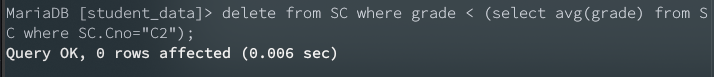
\includegraphics[width=1\textwidth]{ex2-31.png}}
\end{figure}

\section{實驗小結}

此次的實驗加強了我的 SQL 掌握能力,有些題目我真的想了許久一錯再錯才寫出正確的答案。這次的實驗內容也相比實驗一多很多,我每題都自己寫出來並寫成 LaTeX,蠻有成就感的。

\part{實驗三、視圖與完整性約束}

\section{實驗目的}

学习灵活熟练的进行视图的操作,认识视图的作用;掌握完整性控制的方法。

\begin{itemize}
    \item 熟悉和掌握对数据表中视图的定义操作和SQL命令的使用。
    \item 熟悉和掌握对数据表中视图的查询操作和SQL命令的使用。
    \item 熟悉和掌握对数据表中视图的更新操作和SQL命令的使用,并注意视图更新与基本表更新的区别与联系。
    \item 熟悉SQL语言对数据库进行完整性控制的方法。
\end{itemize}

\section{實驗內容}

\subsection{以S , C , SC表为基础完成以下视图定义及使用}

\begin{itemize}
    \item 定义“SSCH”院学生基本情况视图V\_SSCH。
    \item 将S,C,SC表中学生的学号,姓名,课程号,课程名,成绩定义为视图V\_S\_C\_G。
    \item 将各院学生人数,平均年龄定义为视图V\_NUM\_AVG。
    \item 将各位学生选修课程的门数及平均成绩定义为视图V\_AVG\_S\_G并查询结果。
    \item 查询平均成绩为90分以上的学生学号、姓名和成绩。
    \item 通过视图V\_SSCH,新增加一个学生记录 ('S12','YAN XI',19, 'SSCH'),并查询结果。
    \item 通过视图V\_SSCH,删除学号为“S12”学生信息,并查询结果。
    \item 将视图V\_SSCH中学号为“S12”的学生改名“中南人”。
\end{itemize}

\subsection{使用SQL进行数据完整性控制:包括三类完整性、check短语、constrain子句}

1. 在创建下列关系表时完成如下约束:定义实体完整性;参照完整性(外码、在删除S中的元组时级联删除SC中相应元组、当更新S中的Sno时同时更新SC中的Sno);用户定义完整性:学生年龄<30。

2. 修改S中的约束条件,学号在100-1000之间。

学生关系表 S:

\begin{figure}[H] % H 為當前位置,!htb 為忽略美學標準,htbp 為浮動圖片
    \centering % 圖片居中
    \subfigure[学生关系表S]{
    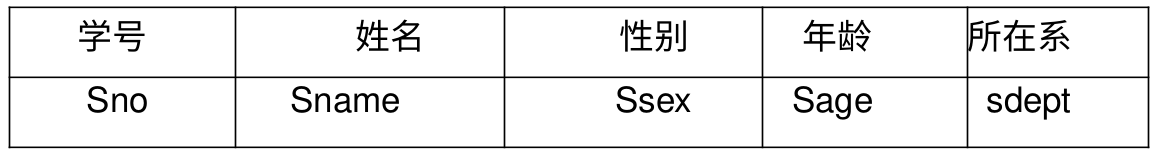
\includegraphics[width=1\textwidth]{ex3-1.png}}
\end{figure}

创建课程关系表 C:

\begin{figure}[H] % H 為當前位置,!htb 為忽略美學標準,htbp 為浮動圖片
    \centering % 圖片居中
    \subfigure[课程关系表C]{
    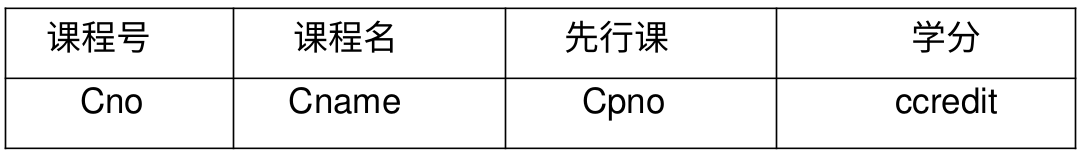
\includegraphics[width=0.75\textwidth]{ex3-2.png}}
\end{figure}

创建学生-课程表SC:

\begin{figure}[H] % H 為當前位置,!htb 為忽略美學標準,htbp 為浮動圖片
    \centering % 圖片居中
    \subfigure[课程关系表C]{
    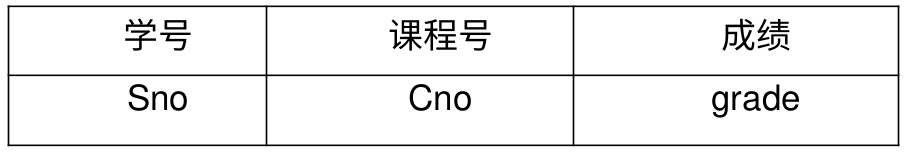
\includegraphics[width=0.75\textwidth]{ex3-3.png}}
\end{figure}

3.用实验验证当操作违反了完整性约束时,系统如何处理?

问题:外键与参照主键是否一定要相同?

\section{實驗方法與實驗步驟}

\begin{itemize}
    \item 定义视图、对视图进行查询、修改。
    \item 进行完整性约束定义、修改。
    \item 进行约束违例验证。
\end{itemize}

\section{實驗結果}

\subsection{View 的基本操作}

1. 定义“SSCH”院学生基本情况视图V\_SSCH。\\

\begin{lstlisting}[language=SQL]
    create view V_SSCH as select * from S where S.sdept = "SSCH";
\end{lstlisting}

\begin{figure}[H] % H 為當前位置,!htb 為忽略美學標準,htbp 為浮動圖片
    \centering % 圖片居中
    \subfigure[創建 V\_SSCH]{
    \includegraphics[width=1\textwidth]{ex3-4.png}}
\end{figure}

\begin{figure}[H] % H 為當前位置,!htb 為忽略美學標準,htbp 為浮動圖片
    \centering % 圖片居中
    \subfigure[插入新數據]{
    \includegraphics[width=0.75\textwidth]{ex3-5.png}}
\end{figure}

\begin{figure}[H] % H 為當前位置,!htb 為忽略美學標準,htbp 為浮動圖片
    \centering % 圖片居中
    \subfigure[查看 View]{
    \includegraphics[width=1\textwidth]{ex3-6.png}}
\end{figure}

%----------------------------------------------------------------------------
2. 将S,C,SC表中学生的学号,姓名,课程号,课程名,成绩定义为视图V\_S\_C\_G。\\

\begin{lstlisting}[language=SQL]
    create or replace view V_S_C_G as select S.Sno, S.Sname, C.Cno, C.Cname, SC.grade from S, C, SC where S.Sno = SC.Sno and C.Cno = SC.Cno;
\end{lstlisting}

\begin{figure}[H] % H 為當前位置,!htb 為忽略美學標準,htbp 為浮動圖片
    \centering % 圖片居中
    \subfigure[V\_S\_C\_G]{
    \includegraphics[width=1\textwidth]{ex3-7.png}}
\end{figure}

{因為發現自己調建設錯了,所以重新更新一次。}

\begin{figure}[H] % H 為當前位置,!htb 為忽略美學標準,htbp 為浮動圖片
    \centering % 圖片居中
    \subfigure[修改 View]{
    \includegraphics[width=1\textwidth]{ex3-8.png}}
\end{figure}

%----------------------------------------------------------------------------
3. 将各院学生人数,平均年龄定义为视图V\_NUM\_AVG。\\

\begin{lstlisting}[language=SQL]
    create view V_NUM_AVG as select S.sdept, count(S.Sno), avg(S.Sage) from S group by S.sdept;
\end{lstlisting}

\begin{figure}[H] % H 為當前位置,!htb 為忽略美學標準,htbp 為浮動圖片
    \centering % 圖片居中
    \subfigure[V\_NUM\_AVG]{
    \includegraphics[width=1\textwidth]{ex3-9.png}}
\end{figure}

%----------------------------------------------------------------------------
4. 将各位学生选修课程的门数及平均成绩定义为视图V\_AVG\_S\_G并查询结果。\\

\begin{lstlisting}[language=SQL]
    create view V_AVG_S_G
    as
    select count(SC.Sno), avg(SC.grade) from SC, C
    where SC.Cno = C.Cno
    group by SC.Sno;
\end{lstlisting}

\begin{figure}[H] % H 為當前位置,!htb 為忽略美學標準,htbp 為浮動圖片
    \centering % 圖片居中
    \subfigure[V\_AVG\_S\_G]{
    \includegraphics[width=1\textwidth]{ex3-10.png}}
\end{figure}

%----------------------------------------------------------------------------
5. 查询平均成绩为90分以上的学生学号、姓名和成绩。\\

\begin{lstlisting}[language=SQL]
    select SC.Sno, S.Sname, SC.grade from SC, S where S.Sno = SC.Sno in (select SC.Sno from SC group by SC.Sno having avg(SC.grade) > 90);
\end{lstlisting}

\begin{figure}[H] % H 為當前位置,!htb 為忽略美學標準,htbp 為浮動圖片
    \centering % 圖片居中
    \subfigure[查詢]{
    \includegraphics[width=1\textwidth]{ex3-11.png}}
\end{figure}

%----------------------------------------------------------------------------
6. 通过视图V\_SSCH,新增加一个学生记录 ('S12','YAN XI',19, 'SSCH'),并查询结果。\\

\begin{lstlisting}[language=SQL]
    insert into V_SSCH(Sno, Sname, Sage, Sdept) values("S12", "YAN XI", 19, "SSCH");
    select * from V_SSCH where Sno="S12";
\end{lstlisting}

\begin{figure}[H] % H 為當前位置,!htb 為忽略美學標準,htbp 為浮動圖片
    \centering % 圖片居中
    \subfigure[新增數據到 V\_SSCH]{
    \includegraphics[width=1\textwidth]{ex3-12.png}}
\end{figure}

%----------------------------------------------------------------------------
7. 通过视图V\_SSCH,删除学号为“S12”学生信息,并查询结果。\\

\begin{lstlisting}[language=SQL]
    delete from V_SSCH where Sno="S12";
    select * from V_SSCH;
\end{lstlisting}

這裡我不小心輸錯了,重輸一遍。

\begin{figure}[H] % H 為當前位置,!htb 為忽略美學標準,htbp 為浮動圖片
    \centering % 圖片居中
    \subfigure[從 V\_SSCH 刪除一筆數據]{
    \includegraphics[width=1\textwidth]{ex3-13.png}}
\end{figure}

%----------------------------------------------------------------------------
8. 将视图V\_SSCH中学号为“S12”的学生改名“中南人”。\\

\begin{lstlisting}[language=SQL]
    update V_SSCH set Sno="中南人" where Sno="S12";
\end{lstlisting}

\begin{figure}[H] % H 為當前位置,!htb 為忽略美學標準,htbp 為浮動圖片
    \centering % 圖片居中
    \subfigure[從 V\_SSCH 更新一筆數據]{
    \includegraphics[width=1\textwidth]{ex3-14.png}}
\end{figure}

\subsection{数据完整性控制}

\subsubsection{創建約束}

1. 定義實體完整性

添加主鍵約束。

發現自己上個實驗就已經設主鍵了。\\

\begin{lstlisting}[language=SQL]
    alter table S add primary key(Sno);
\end{lstlisting}

\begin{figure}[H] % H 為當前位置,!htb 為忽略美學標準,htbp 為浮動圖片
    \centering % 圖片居中
    \subfigure[S 設 primary key]{
    \includegraphics[width=1\textwidth]{ex3-15.png}}
\end{figure}

試試網上找到的其他寫法,結果報了 Warning,但還是成功了。\\

\begin{lstlisting}[language=SQL]
    alter table C add constraint constraint_c primary key(Cno);
\end{lstlisting}

\begin{figure}[H] % H 為當前位置,!htb 為忽略美學標準,htbp 為浮動圖片
    \centering % 圖片居中
    \subfigure[C 設 primary key]{
    \includegraphics[width=1\textwidth]{ex3-16.png}}
\end{figure}

\begin{lstlisting}[language=SQL]
    alter table SC add  primary key(Sno, Cno);
\end{lstlisting}

\begin{figure}[H] % H 為當前位置,!htb 為忽略美學標準,htbp 為浮動圖片
    \centering % 圖片居中
    \subfigure[SC 設 primary key]{
    \includegraphics[width=1\textwidth]{ex3-17.png}}
\end{figure}
%--------------------------------------------------------
2. 參照完整性

設置外鍵:\\

\begin{lstlisting}[language=SQL]
    alter table SC add foreign key(Sno) references S(Sno);
\end{lstlisting}

因為 SC 有些 Sno 不在父 S 的 Sno 裡所以出現下面第一張圖的錯誤,我將 SC 的資料修一下再次執行就好了。

\begin{figure}[H] % H 為當前位置,!htb 為忽略美學標準,htbp 為浮動圖片
    \centering % 圖片居中
    \subfigure[SC 設 foreign key 失敗]{
    \includegraphics[width=1\textwidth]{ex3-18.png}}
\end{figure}

\begin{figure}[H] % H 為當前位置,!htb 為忽略美學標準,htbp 為浮動圖片
    \centering % 圖片居中
    \subfigure[SC 設 foreign key]{
    \includegraphics[width=1\textwidth]{ex3-19.png}}
\end{figure}

3. 用戶定義完整性

\begin{lstlisting}[language=SQL]
    alter table S add check(Sage < 30);
\end{lstlisting}

\subsubsection{修改約束條件}

\begin{lstlisting}[language=SQL]
    Alter table S add check(Sno between 100 and 1000);
\end{lstlisting}

\section{實驗小結}

這次的實驗讓我學會怎麼給數據庫添加 View,還有主鍵和外鍵,最後也讓我時做了約束條件。我覺得真的有學到的感覺,也對數據庫又更深一步的了解。

\part{實驗一、數據庫與表的基本操作}

\section{實驗目的}



\section{實驗內容}

\section{實驗方法與實驗步驟}

\section{實驗結果}

\section{實驗小結}

\part{實驗一、數據庫與表的基本操作}

\section{實驗目的}



\section{實驗內容}

\section{實驗方法與實驗步驟}

\section{實驗結果}

\section{實驗小結}

\end{document}